\documentclass[tikz,border=5mm]{standalone}
\begin{document}
	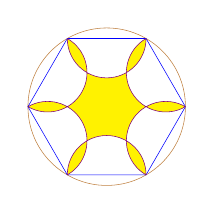
\begin{tikzpicture}[line join=round,very thin]
		\def\r{1}
		\draw[brown] (0,0)coordinate(O) circle (\r);
		\foreach \i in {1,2,...,6}
		\coordinate(A_\i) at (60*\i-60:\r);
		\draw[blue] (A_1)--(A_2)--(A_3)--(A_4)--(A_5)--(A_6)--cycle;
		\filldraw[violet,fill=yellow] (A_1) arc (-60:-240:\r/2)arc (0:-180:\r/2)arc (60:-120:\r/2)arc (120:-60:\r/2)arc (180:0:\r/2)arc (240:60:\r/2);
	\end{tikzpicture}
\end{document}